\newpage
%%%%%%%%%%%%%%%%%%%%%%%%%%%%%%%%%%%%%%%%%%%%%%%%%%%%%%%%%%%%%%%%
%%%%%%%%%%%%%%%%%%%%%%%%%%%%%%%%%%%%%%%%%%%%%%%%%%%%%%%%%%%%%%%%
%%%%%%%%%%%%%%%%%%%%%%%%%% Enunciado %%%%%%%%%%%%%%%%%%%%%%%%%%%

\begin{myblock}
\phantomsection\addcontentsline{toc}{section}{Parte A | GRU}
\section*{Parte A | GRU}

    Entrena los modelos con las canciuones y con las arquitecturas RNN/LSTM/GRU. A nivel
    caracter y a nivel palabra.

\end{myblock}

% \begin{figure}[h!]
%    \centering
%    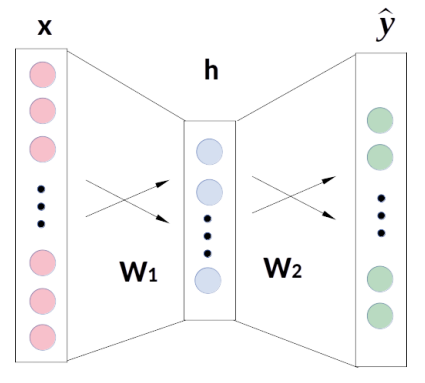
\includegraphics[width=0.4\linewidth]{Images/Red_Problema_02.png}
%    \caption{Red neuronal densamente conectada con una sola capa oculta.}
%    \label{fig:red_p02}
% \end{figure}

%%%%%%%%%%%%%%%%%%%%%%%%%%%%%%%%%%%%%%%%%%%%%%%%%%%%%%%%%%%%%%%%
%%%%%%%%%%%%%%%%%%%%%%%%%%%%%%%%%%%%%%%%%%%%%%%%%%%%%%%%%%%%%%%%

%%%%%%%%%%%%%%%%%%%%%%%%%%%%%%%%%%%%%%%%%%%%%%%%%%%%%%%%%%%%%%%%
%%%%%%%%%%%%%%%%%%%%%%%%%%%%%%%%%%%%%%%%%%%%%%%%%%%%%%%%%%%%%%%%

En el contexto de las RNN, sabemos que estas se mueven sin una ventana fija. El estado oculto $h_t$ resume el pasado y se actualiza con el nuevo $x_t$,. es decir, la palabra en la posición $t$, para predecir la salida $y_t$. En una RNN clásica, el cálculo se organiza en tres bloques: de la capa de entrada al estado oculto, del estado oculto a otro estado oculto, y de ese estado oculto a la salida. El entrenamiento del modleo de lenguaje s ehace por auto-supervisión con entropía cruzada como función objetivo, donde la probabilidad de la secuencia se factoriza paso a paso y se optimiza la pérdida. 

Sin embargo, RNN sufré del desvanecimiento del gradiente. Agregar compuertas como hace la LSTM resuelve ese problema al descartar información y decidir la que sí es de importancia para las decisiones. Dentro de la familia de RNN con compuertas se encuentra también la GRU. 

Conocida como Gated Recurrent Unit (GRU), este tipo de arquitecturas intenta mantener un desempeño competitivo con las LSTM a pesar de introducir menos parámetros. 

\subsection{La célula GRU y sus compuertas}

Una GRU controla el flujo de información con dos compuertas sigmoides por dimensión: la compuerta de actualización $z_t$ y  la compuerta de reinicio llamada $r_t$. La idea clave frente a la LSTM es que una sola compuerta gobierna a la vez el "olvido" del pasado y la decisión de escribir el nuevo estado, simplificando la arquitectura. 

Las ecuaciones de actualización son:

\begin{itemize}
    \item \textbf{Compuerta de actualización}: $z_t = \sigma(b_z + U_z x_t + W_z h_{t-1})$
    \item \textbf{Compuerta de reinicio}: $r_t = \sigma(b_r + U_r x_t + W_r h_{t-1})$
    \item \textbf{Candidato de estado}: $\hat{h}_t = \text{tanh}\Big(b + Ux_t + W(r_t \;\; \odot \;\; h_{t-1})\Big)$
    \item \textbf{Mezcla final}: $h_t = z_t \;\; \odot \;\; h_{t-1} + (1 - z_t) \;\; \odot \;\; \hat{h}_t$ 
\end{itemize}

La intuición detrás de esto es que $z_t$ implementa un integrador con fuga condicional. i.e. cerca de 1 "copia" el estado oculto $h_{t-1}$; mientras que cerca de 0 "reescribe" con $\hat{h}_t$. Por otra parte, $r_t$ decide cuánto del pasado participa en el cómputo del candidato $\hat{h}_t$, introduciendo no linealidad adicional a la relación entre lo pasado y lo futuro. 

A nivel estructural, la GRU mantiene los tres bloques U, W, V de una RNN, pero sustituye la transición oculta a oculta por una transición puerta a dependiente. Al compararse con una LSTM, la GRU elimina el estado de celda explícito y la salida está directamente en $h_t$. De esa manera, intenta ahorrar recursos volviendo a la GRU una LSTM "destilada". Ambos modelos suelen ser competitivos entre ellos, y su uso depende del problema específico a atender. 

\subsection{Arquitectura Utilizada e Hiperparámetros}

Para la tarea de generación de texto se implementó y evaluó un modelo basado en la arquitectura de Unidades Recurrentes Gated (GRU, por sus siglas en inglés). Esta arquitectura fue seleccionada por su eficiencia y su capacidad para capturar dependencias a largo plazo en secuencias, siendo una alternativa robusta a las redes LSTM.

El modelo fue entrenado tanto a nivel de carácter como a nivel de palabra para realizar una comparación exhaustiva. La arquitectura y los hiperparámetros se mantuvieron consistentes entre ambas modalidades para asegurar una evaluación justa de los resultados. A continuación, se detalla la configuración específica utilizada para los modelos GRU.

\subsubsection{Arquitectura del Modelo GRU}

El diseño del modelo se construyó como una pila de capas secuenciales, utilizando el framework \texttt{PyTorch}. La estructura fue la siguiente:

\begin{enumerate}
    \item \textbf{Capa de Embedding:} Una capa inicial que transforma los índices de los tokens (sean caracteres o palabras) en vectores densos. La dimensión de estos vectores de embedding se fijó en 128.

    \item \textbf{Capas GRU Apiladas:} El núcleo del modelo consiste en 4 capas GRU apiladas, cada una con una dimensión de estado oculto (\texttt{hidden\_dim}) de 256 unidades. El apilamiento de capas permite al modelo aprender representaciones de los datos a diferentes niveles de abstracción.

    \item \textbf{Capa de Regularización (Dropout):} Para mitigar el sobreajuste, se aplicó una capa de \texttt{Dropout} entre cada una de las capas GRU, con una tasa de desactivación de neuronas del 30\% (0.3).

    \item \textbf{Capa de Salida (Clasificador):} Finalmente, una capa lineal (densa) proyecta el estado oculto de la última capa GRU al tamaño del vocabulario, seguida de una función de activación \texttt{Softmax} para obtener una distribución de probabilidad sobre el siguiente token a predecir.
\end{enumerate}

\subsubsection{Hiperparámetros de Entrenamiento}

El proceso de entrenamiento fue configurado con los hiperparámetros que se resumen en la Tabla \ref{tab:gru_hyperparams}. La elección de estos valores se basó en una combinación de prácticas estándar y ajustes empíricos para la tarea.

\begin{table}[h!]
    \centering
    \caption{Resumen de hiperparámetros de entrenamiento para el modelo GRU.}
    \label{tab:gru_hyperparams}
    \begin{tabular}{l|l}
        \hline
        \textbf{Hiperparámetro} & \textbf{Valor Utilizado} \\ \hline
        Optimizador & \texttt{Adam} \\
        Tasa de Aprendizaje (Learning Rate) & \texttt{5e-4 (0.0005)} \\
        Función de Pérdida & \texttt{Cross-Entropy Loss} \\
        Tamaño del Lote (Batch Size) & \texttt{32} \\
        Épocas de Entrenamiento & \texttt{15} \\
        Semilla Aleatoria (Seed) & \texttt{42} \\ \hline
    \end{tabular}
\end{table}

\subsection{Resultados}

\begin{lstlisting}[
    style=mystyle,
    caption={Output crudo del modelo GRU a nivel de carácter.},
    label={lst:output-gru-char}
]
I <UNK> <UNK> <UNK> <UNK> <UNK> <UNK> <UNK>  v i s p e n s e  a n d  a b o v e  m y  t h r o a t ?  S h a d o w s  w i l l  s c r e a m  t h a t  I ' m  a l o n e - l o n e - l o n e  I - I - I - I ' v e  g o t  a  m i g r a i n e  A n d  m y  p a i n  w i l l  r a n g e  f r o m  u p ,  d o w n ,  a n d  s i d e w a y s  T h a n k  G o d  i t ' s  F r i d a y  ' c a u s e  F r i d a y s  w i l l  a l w a y s  b e  o n  a  s o n g  h e  w r o t e  T h i s  i s  t h e  l a s t  t i m e ,  t h i s  i s  t h e  l a s t  t i m e ,  t h i s  i s  t h e  l a s t  t i m e ,  t h i s  i s  t h e  l a s t  t i m e ,  t h i s  i s  t h e  l a s t  t i m e  E n t e r t a i n  m y  f a i t h  T h i s  i s  t h e  l a s t  t i m e ,  t h i s  i s  t h e  l a s t  t i m e
\end{lstlisting}

\begin{lstlisting}[
    style=mystyle,
    caption={Output crudo del modelo GRU a nivel de palabra.},
    label={lst:output-gru-word}
]
<UNK> like my soul but not my mind have i have back when a beautiful day but you me, around they will never don't want to know you who i see do i will you'll don't take a piece, of gold? to someone tryin' all next like what i wanna your footing, of nothing but i am i'll keep movin' a last feeling that come in black it's now what i know, up they get cold, sitting i get down) i get it's they just get to be all you never have it again never know they morph of a kingdom, join did a concert, i'll decorates with instead is a good progression catch i don't know i had to do one on my pride lean on my pride, i'm a lion i should the count i know the gesture we be slow i sing a day for break with a little cheetah after a re-beginning moment's mending memories dormant the beeps and tones keep would that not be 'cause me, are frozen and the mainland is climbing flying but we can the picture (am then my shirtsleeve shadows jacket not your wits then you mine to subliminally get out start (ooh-ooh) i don't go through you don't
\end{lstlisting}


\subsection{Conclusiones}

El modelo GRU mostró un comportamiento intermedio entre la simplicidad de la RNN y la capacidad
de memoria extendida de la LSTM. El comportamiento de la PPL demostró que, para este modelo 
de GRU, a nivel carácter descendió rápidamente hasta estabilizarse en valores bajos, los 
cuales fueron comparables con los alcanzados por la LSTM. En cuanto al texto generado, mostró
patrons fonéticos precisos y estructuras repetitivas con ritmo lírico, así como la toma de 
secuencias reconocibles de Twenty One Pilots como ``\textit{Shadows will scream that I'm alone}''
o ``\textit{I've got a migraine}'' de Holding On To You y de Migraine, ambas canciones muy populares 
de la banda. Esto demuestra que el modelo estaba un tanto limitado en cuanto a la creatividad,
pero que lograba encontrar secuencias líricas de importancia. 

Respecto a los resultados de la GRU a nivel palabra, la PPL mostró una disminución constante
hasta valoers relativamente bajos, aunque superiores a los alcanzados por la LSTM. Los outputs
generados reflejaron cierta coherencia temática, con construcciones gramticales mśa estbales que
las obtenidas por la RNN. Se observaron frases como ``\textit{i'll keep movin}''
o ``\textit{they morph of a kingdom}'', que si bien tenían una semántica clara, no se conectaban
del todo bien entre ellas. Esto refleja que nuestra GRU logra capturar contexto de medio alcance, 
que tiene dificultades con alcanzar la fluidez global de una LSTM. 

Los resultados de novelty confirman lo anterior. La GRU obtuvo una novedad en trigamas de 0.92,
la más alta en nuestros tres modelos de redes neuronales, pero en bigramas una de solo 0.62. Esto
nos parece estar diciendo que la arquitectura es especialmente efectiva para evitar repetición 
de manera excesiva, y explorar combinaciones nuevas sin sacrificar del todo la coherencia. Al 
compararlo con la RNN, se mostró una mayor memorización, mientras que el LSTM demuestra un balance
más equilibrado entre memoria novedad. 

De ese modo, podemos decir que la GRU es un modelo que cae justo en medio de la simpleza de la
RNN y sus problemas de memorización, y el entendimiento global y complejo de la LSTM. Es competivia
con la LSTM y supera claramente a la RNN. Quizás un modelo mejor regularizado, con un corpus 
más amplio y más tiempo de cómputo pueda demostrar ser una alternativa clara y eficaz a la LSTM.


%%%%%%%%%%%%%%%%%%%%%%%%%%%%%%%%%%%%%%%%%%%%%%%%%%%%%%%%%%%%%%%%
%%%%%%%%%%%%%%%%%%%%%%%%%%%%%%%%%%%%%%%%%%%%%%%%%%%%%%%%%%%%%%%

\clearpage